

%Portada del Documento
\chapter{Android}
\setlength{\unitlength}{1 cm} %Especificar unidad de trabajo
\thispagestyle{empty}
\begin{picture}(18,8)
\put(5,0){
\includegraphics[width=4cm,height=5cm]{./imagenes3/logo.png}}
\end{picture}
\begin{center}

\end{center}



% fin de la portada


\newpage
\section{ Introducción}

La aplicación realizada con la finalidad de ayudar al usuario a llevar un mejor control de sus facturas. Está aplicación esta dirigida  para personas naturales no obligadas a llevar contabilidad que deben cumplir que tienen problemas al momento de llevar el control de sus facturas para declaraciones de Gastos Personales en el SRI (Servicio de Rentas Internas).
La aplicación recordará al usuario las fechas que le toca hacer sus declaraciones al SRI según el informe que se ha generado al llevar la contabilidad de las facturas que se ha ido guardando.
    \subsection{ Requisitos}
\begin{itemize}
\item Eclipse IDE for Java Developers
\item Descargar el SDK de Android.
\item Plugin Android para Eclipse.
\end{itemize}


\begin{figure}[ht!]
 
   \centering
   %%----primera subfigura----
   \subfloat[]{
        \label{fig:pantalla:1}         %% Etiqueta para la primera subfigura
        
\includegraphics[width=0.42\textwidth]{./imagenes3/img1.png}}
   \hspace{0.1\linewidth}
   %%----segunda subfigura----
   \subfloat[]{
        \label{fig:pantalla:2}         %% Etiqueta para la segunda subfigura
        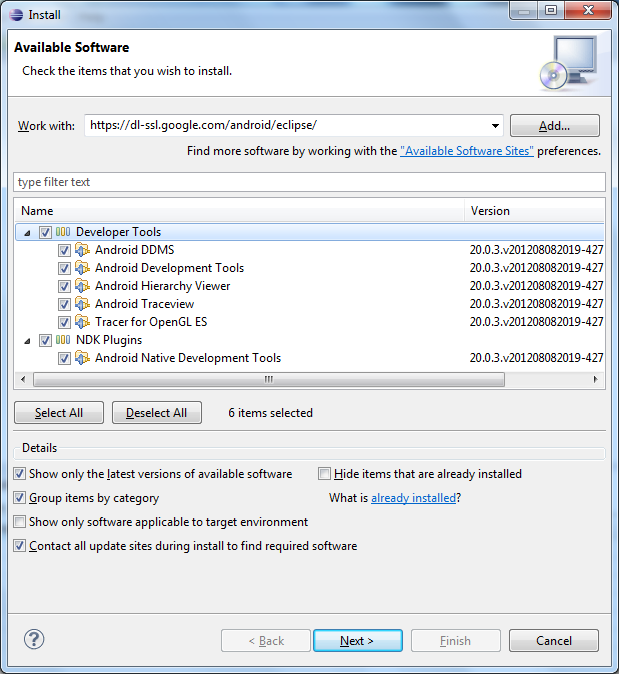
\includegraphics[width=0.42\textwidth]{./imagenes3/img2.png}}\\[20pt]
   %%----tercera subfigura----
   \subfloat[]{
        \label{fig:pantalla:3}         %% Etiqueta para la tercera subfigura
        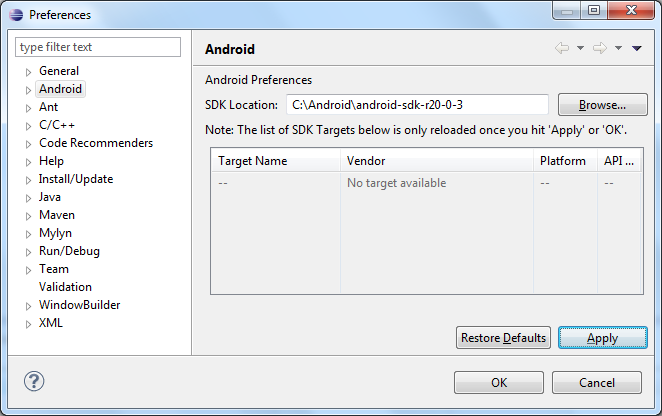
\includegraphics[width=0.42\textwidth]{./imagenes3/img3.png}}
    
\end{figure}


\section{ Como ejecutar el proyecto}
Primero copiamos el archivo del proyecto en cualquier directorio, luego abrimos Ecplipse , seguimos los siguientes pasos:
\begin{enumerate}
\item Dar click Archivo -> Abrir Proyecto y buscamos la carpeta del proyecto en el directorio que lo guardamos.
\item Luego en la barra de herramientas dar click en ejecutar.
\end{enumerate}
     
\begin{figure}[ht!]
 
   \centering
   %%----primera subfigura----
   \subfloat[]{
        \label{fig:pantalla:1}         %% Etiqueta para la primera subfigura
        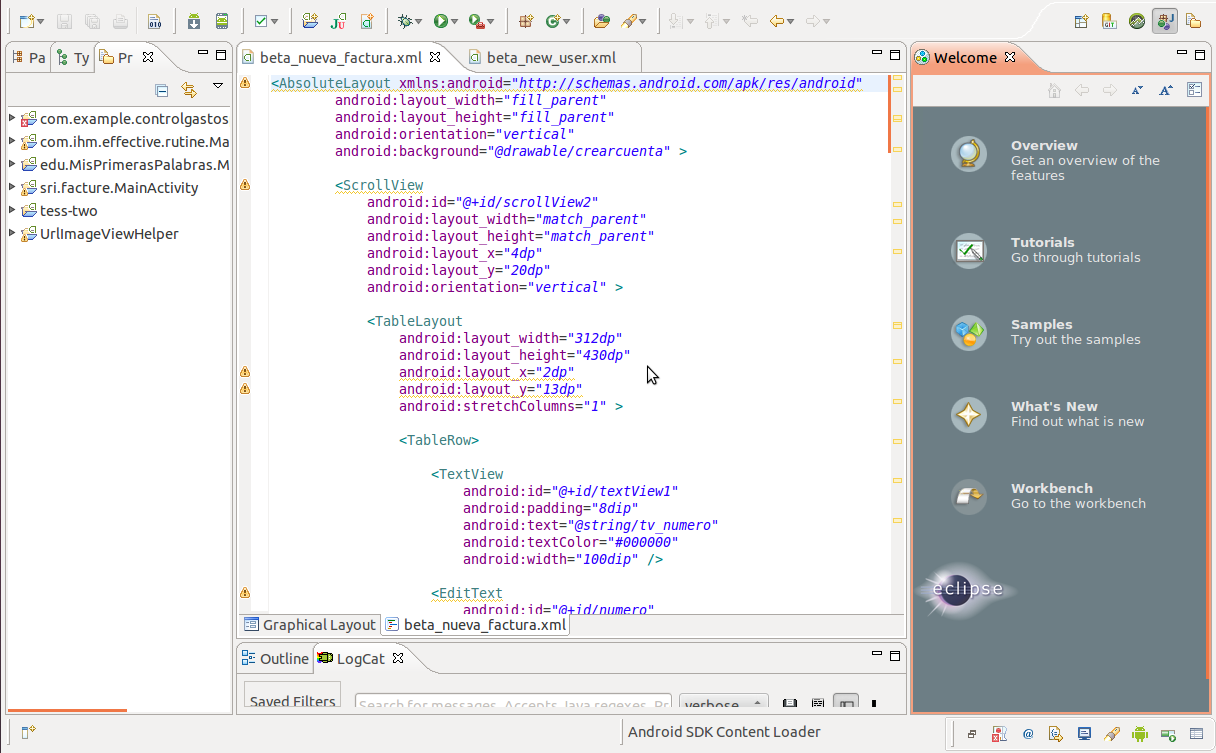
\includegraphics[width=0.42\textwidth]{./imagenes3/img4.png}}
   \hspace{0.1\linewidth}
   %%----segunda subfigura----
   \subfloat[]{
        \label{fig:pantalla:2}         %% Etiqueta para la segunda subfigura
        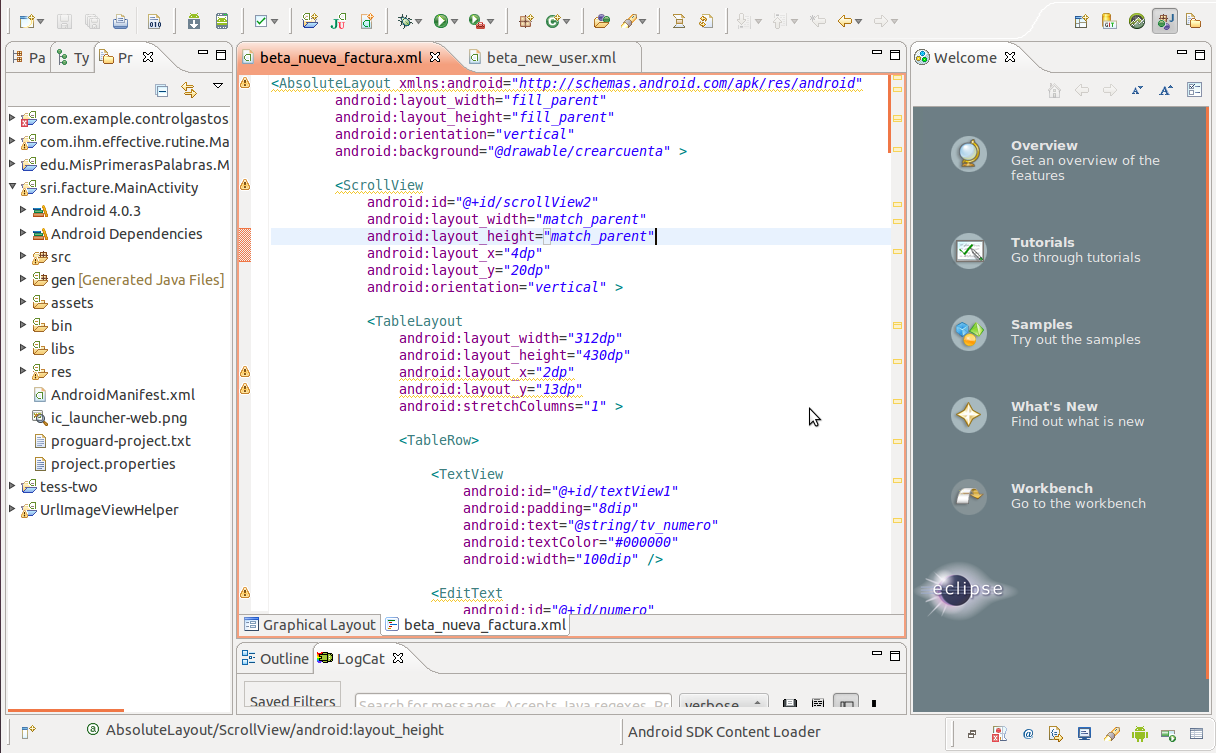
\includegraphics[width=0.42\textwidth]{./imagenes3/img5.png}}
  
\end{figure}

 
\section{ Aplicación}
A continuación se muestran algunas imagenes de  cada una de las pantallas de la aplicación
\begin{enumerate}[a)]
     \item  El emulador cargandose
     \item Aparece el logo de la aplicacion .
     \item La primera ventana donde se ingresa el usuario y la contraseña
    \item Datos de usuario
    

\end{enumerate}

\begin{figure}[ht!]

   \centering     %%----primera subfigura----
   \subfloat[]{
        \label{fig:pantalla:1}         %% Etiqueta para la primera subfigura
        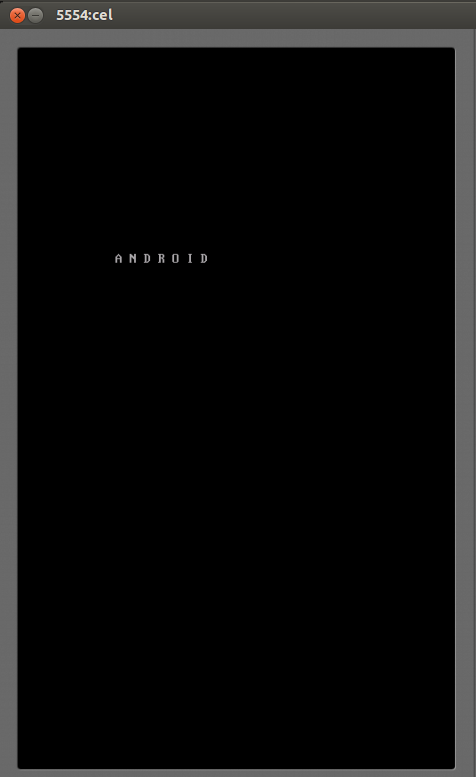
\includegraphics[width=0.42\textwidth]{./imagenes3/img6.png}}
   \hspace{0.1\linewidth}
   %%----segunda subfigura----
   \subfloat[]{
        \label{fig:pantalla:2}         %% Etiqueta para la segunda subfigura
        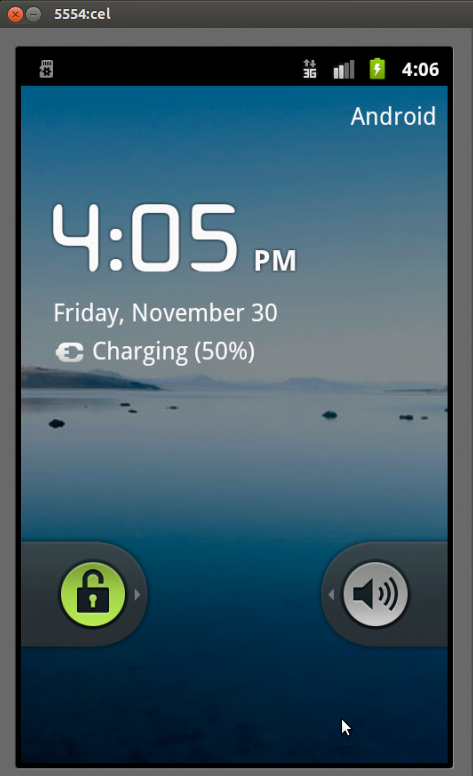
\includegraphics[width=0.42\textwidth]{./imagenes3/img7.png}}\\[20pt]
   %%----tercera subfigura----
   \subfloat[]{
        \label{fig:pantalla:3}         %% Etiqueta para la tercera subfigura
        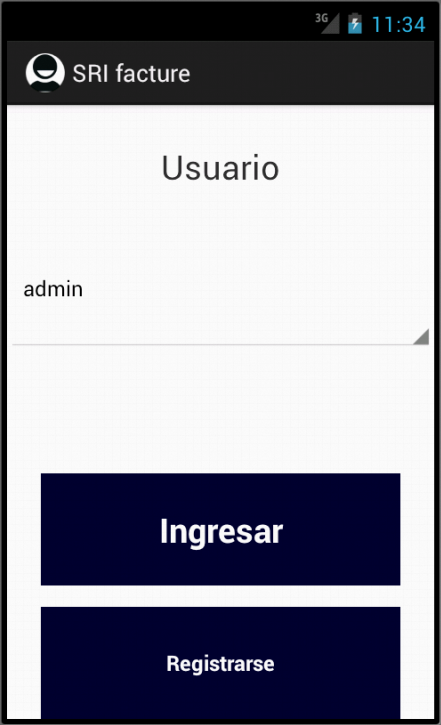
\includegraphics[width=0.42\textwidth]{./imagenes3/img8.png}}
    \hspace{0.1\linewidth}
   %%----cuarta subfigura----
    \subfloat[]{
        \label{fig:pantalla:4}         %% Etiqueta para la cuarta subfigura
        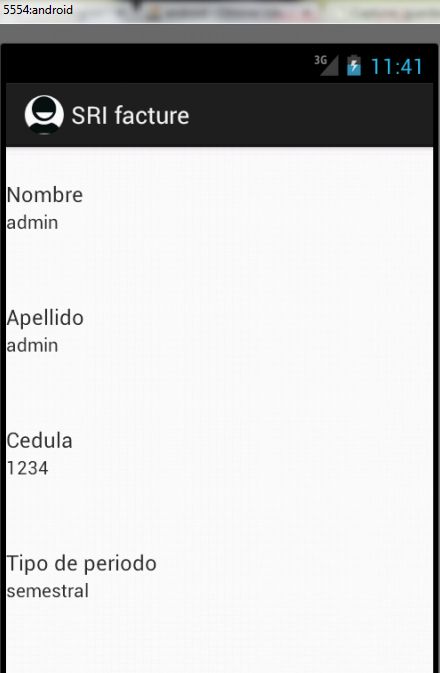
\includegraphics[width=0.42\textwidth]{./imagenes3/img13.png}}
\end{figure}

\begin{enumerate}[a)]
       \item El menu de la aplicación.
    \item Se puede ver la pantalla donde se ingresa a abministrar factura.
       \item  En esta pantalla se muestran los diferentes valores guardados 
     \item Reporte .   
\end{enumerate}

\begin{figure}[ht!]
   \centering
   %%----primera subfigura---- \
\subfloat[]{
        \label{fig:pantalla:3}         %% Etiqueta para la tercera subfigura
        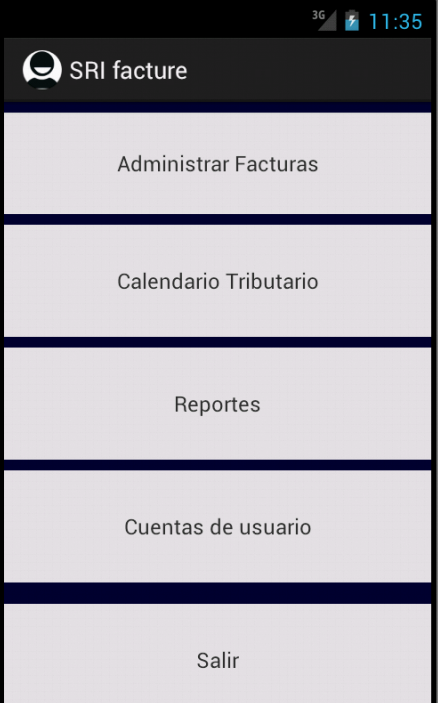
\includegraphics[width=0.42\textwidth]{./imagenes3/img9.png}}
\hspace{0.1\linewidth}
   \subfloat[]{
        \label{fig:pantalla:1}         %% Etiqueta para la primera subfigura
        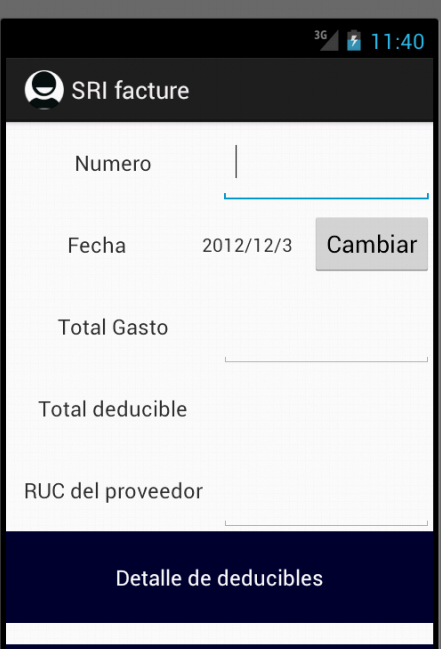
\includegraphics[width=0.42\textwidth]{./imagenes3/img11.png}}\\[20pt]
  
   %%----segunda subfigura----
   \subfloat[]{
        \label{fig:pantalla:2}         %% Etiqueta para la segunda subfigura
        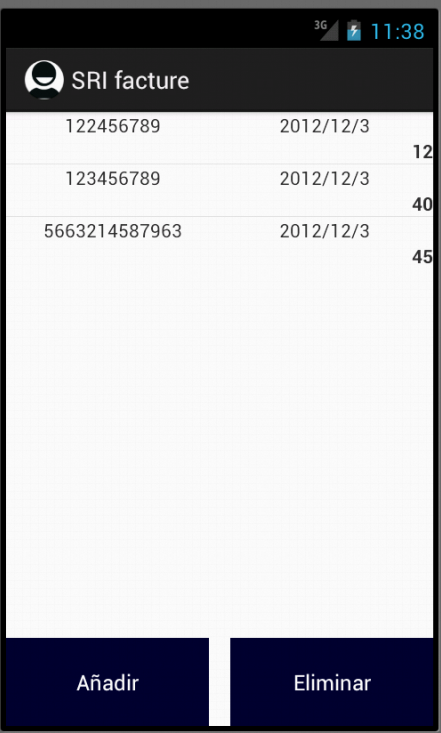
\includegraphics[width=0.42\textwidth]{./imagenes3//img10.png}}
\hspace{0.1\linewidth}
   %%----tercera subfigura----
   \subfloat[]{
        \label{fig:pantalla:3}         %% Etiqueta para la tercera subfigura
        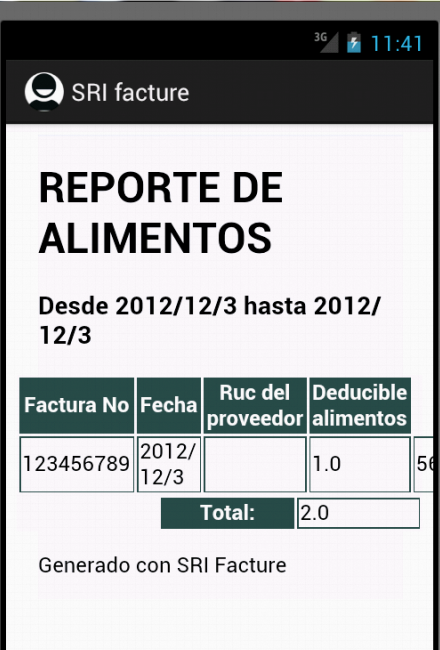
\includegraphics[width=0.42\textwidth]{./imagenes3/img12.png}}
   
\end{figure}

\section{ Experiencias}
 Esta experiencia ha mostrado cómo es posible diseñar y aplicar lo que hemos aprendido en anteriores curso complementado con la investigación que se realizó.
\begin{itemize}
\item En el entorno que será util la aplicación será según el lugar de encuentro del usuario en el momento de tener la factura en sus manos, porque de esta manera el usario el usuario podrá llevar un registro de sus facturas en caso de que pierda una.
\item Una observación muy importante es que nuestra aplicacion tiene uso solo para Ecuador, aunque se podria hacer cambios para  que se adapte otros paises 
\item Mediante las pruebas realizadas, los problemas que tuvieron  mayor frecuencia son:
  \begin{itemize}
\item Problemas para regresar en la aplicación.
\item Problemas para visualizar la opción de Crear Cuenta.
\item Problemas con  la información de los reportes.
   \end{itemize}
\end{itemize}



